%% Nivio: 21/jan/06
% Time-stamp: <Monday 30 Jan 2006 03:57:28am EDT yoshi@ime.usp.br>
\vspace{-2mm}
\subsection{Partitioning step}
\label{sec:partitioning-keys}

The set $S$ of $n$ keys is partitioned into $\lceil n/b \rceil$ buckets, 
where $b$ is a suitable parameter chosen to guarantee
that each bucket has at most 256 keys with high probability
(see Section~\ref{sec:determining-b}).
The partitioning step works as follows:

\begin{figure}[h]
\hrule 
\hrule 
\vspace{2mm}
\begin{tabbing}
aa\=type booleanx \==  (false, true); \kill
\> $\blacktriangleright$ Let $\beta$ be the size in bytes of the set $S$ \\ 
\> $\blacktriangleright$ Let $\mu$ be the size in bytes of an a priori reserved \\
\> ~~~ internal memory area \\ 
\> $\blacktriangleright$ Let $N = \lceil \beta/\mu \rceil$ be the number of key blocks that will \\
\> ~~~ be read from disk into an internal memory area \\
\> $\blacktriangleright$ Let $\mathit{size}$ be a vector that stores the size of each bucket \\
\> $1.$ {\bf for} $j = 1$ {\bf to} $N$ {\bf do} \\
\> ~~ $1.1$ Read block $B_j$ of keys from disk \\
\> ~~ $1.2$ Cluster $B_j$ into $\lceil n/b \rceil$ buckets using a bucket sort \\
\> ~~~~~~~ algorithm and update the entries in the vector {\it size} \\
\> ~~ $1.3$ Dump $B_j$ to the disk into File $j$\\
\> $2.$ Compute the {\it offset} vector and dump it to the disk.
\end{tabbing}
\hrule 
\hrule 
\vspace{-1.0mm}
\caption{Partitioning step}
\vspace{-3mm}
\label{fig:partitioningstep}
\end{figure}

Statement 1.1 of the {\bf for} loop presented in Figure~\ref{fig:partitioningstep} 
reads sequentially all the keys of block $B_j$ from disk into an internal area
of size $\mu$.

Statement 1.2 performs an indirect bucket sort of the keys in block $B_j$
and at the same time updates the entries in the vector {\em size}.
Let us briefly describe how~$B_j$ is partitioned among the~$\lceil n/b\rceil$
buckets. 
We use a local array of $\lceil n/b \rceil$ counters to store a 
count of how many keys from $B_j$ belong to each bucket.
%At the same time, the global vector {\it size} is computed based on the local 
%counters. 
The pointers to the keys in each bucket $i$, $0 \leq i < \lceil n/b \rceil$,
are stored in contiguous positions in an array.
For this we first reserve the required number of entries
in this array of pointers using the information from the array of counters. 
Next, we place the pointers to the keys in each bucket into the respective
reserved areas in the array (i.e., we place the pointers to the keys in bucket 0, 
followed by the pointers to the keys in bucket 1, and so on).

\enlargethispage{2\baselineskip}
To find the bucket address of a given key
we use the universal hash function $h_0(k)$~\cite{j97}.
Key~$k$ goes into bucket~$i$, where
%Then, for each integer $h_0(k)$ the respective bucket address is obtained
%as follows:
\begin{eqnarray} \label{eq:bucketindex}
i=h_0(k) \bmod \left \lceil \frac{n}{b} \right \rceil.
\end{eqnarray}

Figure~\ref{fig:brz-partitioning}(a) shows a \emph{logical} view of the
$\lceil n/b \rceil$ buckets generated in the partitioning step.
%In this case, the keys of each bucket are put together by the pointers to
%each key stored 
%in contiguous positions in the array of pointers.
In reality, the keys belonging to each bucket are distributed among many files,
as depicted in Figure~\ref{fig:brz-partitioning}(b).
In the example of Figure~\ref{fig:brz-partitioning}(b), the keys in bucket 0 
appear in files 1 and $N$, the keys in bucket 1 appear in files 1, 2
and $N$, and so on. 

\vspace{-7mm}
\begin{figure}[ht]
\centering
\begin{picture}(0,0)%
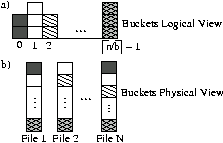
\includegraphics{figs/brz-partitioning.ps}%
\end{picture}%
\setlength{\unitlength}{4144sp}%
%
\begingroup\makeatletter\ifx\SetFigFont\undefined%
\gdef\SetFigFont#1#2#3#4#5{%
  \reset@font\fontsize{#1}{#2pt}%
  \fontfamily{#3}\fontseries{#4}\fontshape{#5}%
  \selectfont}%
\fi\endgroup%
\begin{picture}(4371,1403)(1,-6977)
\put(333,-6421){\makebox(0,0)[lb]{\smash{{\SetFigFont{7}{8.4}{\familydefault}{\mddefault}{\updefault}0}}}}
\put(545,-6421){\makebox(0,0)[lb]{\smash{{\SetFigFont{7}{8.4}{\familydefault}{\mddefault}{\updefault}1}}}}
\put(759,-6421){\makebox(0,0)[lb]{\smash{{\SetFigFont{7}{8.4}{\familydefault}{\mddefault}{\updefault}2}}}}
\put(1539,-6421){\makebox(0,0)[lb]{\smash{{\SetFigFont{7}{8.4}{\familydefault}{\mddefault}{\updefault}${\lceil n/b\rceil - 1}$}}}}
\put(541,-6676){\makebox(0,0)[lb]{\smash{{\SetFigFont{7}{8.4}{\familydefault}{\mddefault}{\updefault}Buckets Logical View}}}}
\put(3547,-6120){\makebox(0,0)[lb]{\smash{{\SetFigFont{12}{14.4}{\familydefault}{\mddefault}{\updefault}.}}}}
\put(3547,-6188){\makebox(0,0)[lb]{\smash{{\SetFigFont{12}{14.4}{\familydefault}{\mddefault}{\updefault}.}}}}
\put(3547,-6255){\makebox(0,0)[lb]{\smash{{\SetFigFont{12}{14.4}{\familydefault}{\mddefault}{\updefault}.}}}}
\put(3107,-6120){\makebox(0,0)[lb]{\smash{{\SetFigFont{12}{14.4}{\familydefault}{\mddefault}{\updefault}.}}}}
\put(3107,-6188){\makebox(0,0)[lb]{\smash{{\SetFigFont{12}{14.4}{\familydefault}{\mddefault}{\updefault}.}}}}
\put(3107,-6255){\makebox(0,0)[lb]{\smash{{\SetFigFont{12}{14.4}{\familydefault}{\mddefault}{\updefault}.}}}}
\put(4177,-6224){\makebox(0,0)[lb]{\smash{{\SetFigFont{12}{14.4}{\familydefault}{\mddefault}{\updefault}.}}}}
\put(4177,-6269){\makebox(0,0)[lb]{\smash{{\SetFigFont{12}{14.4}{\familydefault}{\mddefault}{\updefault}.}}}}
\put(4177,-6314){\makebox(0,0)[lb]{\smash{{\SetFigFont{12}{14.4}{\familydefault}{\mddefault}{\updefault}.}}}}
\put(3016,-6721){\makebox(0,0)[lb]{\smash{{\SetFigFont{7}{8.4}{\familydefault}{\mddefault}{\updefault}File 1}}}}
\put(3466,-6721){\makebox(0,0)[lb]{\smash{{\SetFigFont{7}{8.4}{\familydefault}{\mddefault}{\updefault}File 2}}}}
\put(4096,-6721){\makebox(0,0)[lb]{\smash{{\SetFigFont{7}{8.4}{\familydefault}{\mddefault}{\updefault}File N}}}}
\put(3196,-6946){\makebox(0,0)[lb]{\smash{{\SetFigFont{7}{8.4}{\familydefault}{\mddefault}{\updefault}Buckets Physical View}}}}
\end{picture}%
\caption{Situation of the buckets at the end of the partitioning step: (a) Logical view (b) Physical view}
\label{fig:brz-partitioning}
\vspace{-2mm}
\end{figure}

This scattering of the keys in the buckets could generate a performance
problem because of the potential number of seeks  
needed to read the keys in each bucket from the $N$ files in disk 
during the searching step. 
But, as we show later in Section~\ref{sec:analytcal-results}, the number of seeks 
can be kept small using buffering techniques.
Considering that only the vector {\it size}, which has $\lceil n/b \rceil$
one-byte entries (remember that each bucket has at most 256 keys),
must be maintained in main memory during the searching step,
almost all main memory is available to be used as disk I/O buffer.

The last step is to compute the {\it offset} vector and dump it to the disk.
We use the vector $\mathit{size}$ to compute the
$\mathit{offset}$ displacement vector. 
The $\mathit{offset}[i]$ entry contains the number of keys 
in the buckets $0, 1, \dots, i-1$.
As {\it size}$[i]$ stores the number of keys
in bucket $i$, where $0 \leq i <\lceil n/b \rceil$, we have
\begin{displaymath}
\mathit{offset}[i] = \sum_{j=0}^{i-1} \mathit{size}[j] \cdot
\end{displaymath}
 
